\documentclass[mathserif]{beamer}

\usepackage{amsmath, amssymb}
\usepackage{multicol}

\setbeamertemplate{note page}[plain]
%\setbeameroption{show only notes}

\title[DM Optimizer]{Difference Map Optimizer}
\subtitle{A deterministic method for global unconstrained optimization of
    nonconvex multivariate scalar functions}
\author{Jacob Errington}
\date{20 March 2015}

\renewcommand{\vec}{\mathbf}

\begin{document}

\frame{\titlepage}

\begin{frame}
    \frametitle{Why optimization?}
    \begin{itemize}
        \item Optimization is the bottleneck in a lot of applications.
        \item Current optimizers may require a lot of tweaking.
    \end{itemize}
\end{frame}

\begin{frame}
    \frametitle{Goals}
    $$
    \min_{\vec x \in \mathbb{R}^n} f(\vec x)
    $$
    \begin{itemize}
        \item Works \emph{out of the box}.
            \note[item]{i.e. with as little tweaking as possible.}

        \item Is general.
            \note[item]{Applies to a wide range of problem, e.g. the difference
            map constraint satisfaction algorithm is used for x-ray
            crystallography, sphere packing, and solving sudoku.}

        \item Is comparable to or better than the state-of-the-art.
            \note[item]{The state-of-the-art being Simulated Annealing, due to
            its generality.}

        \item Lets us explore new methods for optimization.
            \note[item]{Existing methods for optimization tend to use stochastic
            processes to achieve good performance. Introducing a certain degree
            of randomness allows these methods to avoid becoming trapped in
            local minima. Deterministic methods are interesting in their own
            right, in some sense, since they aren't used as much.}
    \end{itemize}
\end{frame}

\begin{frame}
    \frametitle{Background: Difference Map constraint satisfaction}

    \note[item]{Why talk about the difference map? It will allow me to make
    references to it later when talking about the DMO algorithm, and in
    particular the intuition for why it should work.}

    \begin{align*}
        P_1 &: X \to C_1 \subset X \\
        P_2 &: X \to C_2 \subset X
    \end{align*}
    \begin{align*}
        \vec x_{n+1} = f(\vec x_n) &= \vec x_n + \beta \left(P_1 (f_2(\vec x_n)) - P_2(f_1(\vec x_n))\right) \\
        f_1(\vec x_n) &= \left(1 - \frac{1}{\beta}\right) P_1(\vec x_n) + \frac{1}{\beta} \vec x_n \\
        f_2(\vec x_n) &= \left(1 + \frac{1}{\beta}\right) P_2(\vec x_n) - \frac{1}{\beta} \vec x_n
    \end{align*}

    \note[item]{Difference map solves constraint satisfaction problems involving two
    constraints, $C_1$ and $C_2$, having associated projection operators $P_1$
    and $P_2$.}
    \note[item]{It's an iterative process, which stops when $f$ reaches a fixed
    point. Project onto one constraint and the other separately, go a little
    bit further ($\beta$), and then use the displacement between the
    projections to move over the iterate.}
    \note[item]{The solution to the problem is always a fixed point of this
    map, but there can be many addition fixed points that are not solutions.}
\end{frame}

\begin{frame}
    \frametitle{Background: Difference Map in action -- 2D}

    A super easy example.
    \begin{center}
        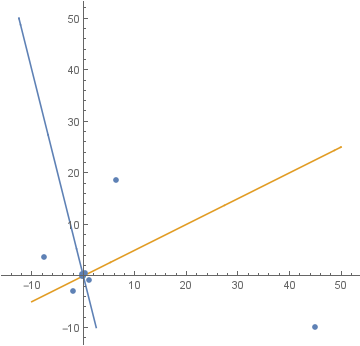
\includegraphics[height=7cm]{../figures/difference-map-pure.png}
    \end{center}
\end{frame}

\begin{frame}
    \frametitle{Background: Difference Map in action -- 3D}

    A non-solution fixed-point is found.
    \begin{center}
        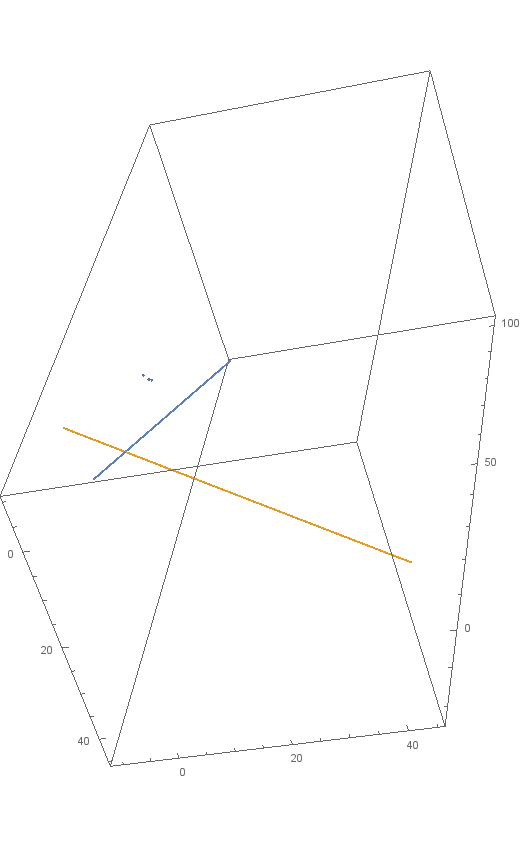
\includegraphics[height=7cm]{../figures/difference-map-3d-fail.png}
    \end{center}
\end{frame}

\begin{frame}
    \frametitle{The DM optimizer: case study -- Griewank function}

    \note[item]{Start with two initial guesses. The first will be considered
    the first local minimum. After performing a local minimzation starting at
    the first guess, we will have two local minima. The second guess is used as
    the starting position for the iterate, which keeps a certain distance from
    the discovered minima}
    \note[item]{Come up with the initial target value. Several ways to
    do this: use the difference between the two initial minima, scaled by some
    constant, to push down from the smaller of the two; use the local smaller
    of the two and just scale it. The former is a more robust solution since it
    isn't biased towards zero.}

    \begin{center}
        \only<1>{
            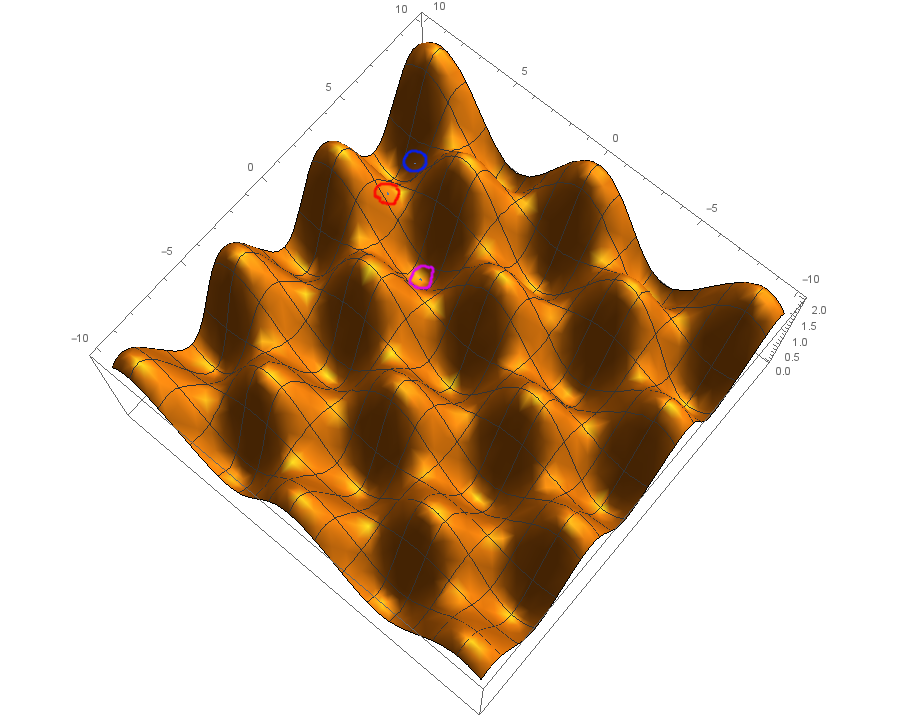
\includegraphics[height=7cm]
                {../figures/griewank-starting-points.png}
        }
        %\only<2>{
        %    \includegraphics[height=7cm]
        %        {../figures/griewank-interating.png}
        %}
    \end{center}
\end{frame}

\begin{frame}
    \frametitle{The Difference Map optimizer: iterating}

    \begin{center}
        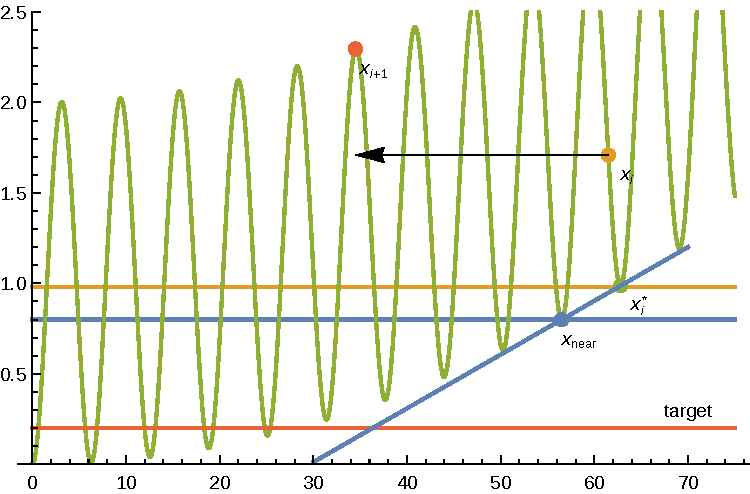
\includegraphics[height=7cm]{../figures/iterating.png}
    \end{center}
\end{frame}

\begin{frame}[allowframebreaks]
    \frametitle{The tested objective functions.}

    \begin{center}
        Griewank.

        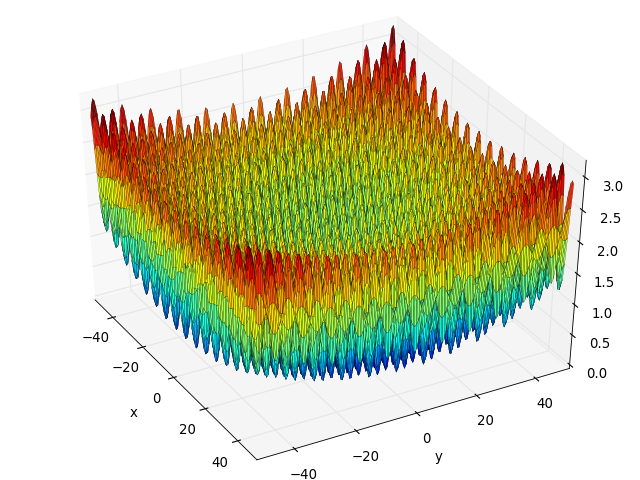
\includegraphics[height=7cm]{../figures/griewank.png}
    \end{center}

    \begin{center}
        Ackley.

        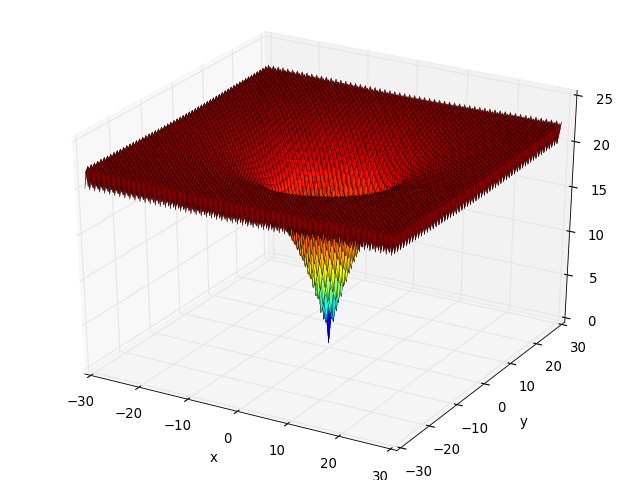
\includegraphics[height=7cm]{../figures/ackley.png}
    \end{center}

    \begin{center}
        Schaffer.

        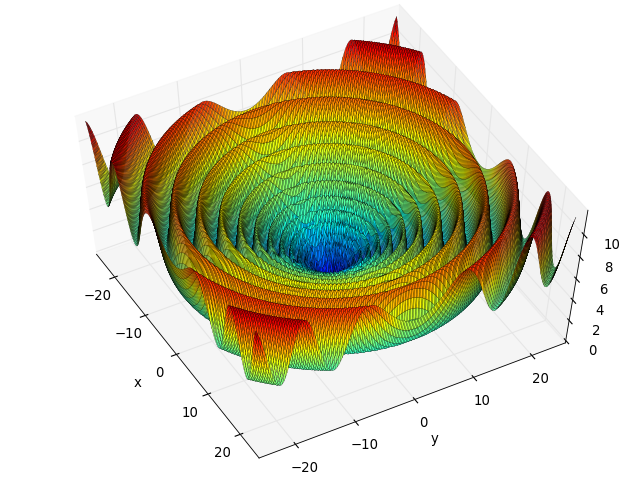
\includegraphics[height=7cm]{../figures/schaffer.png}
    \end{center}

    \begin{center}
        Rosenbrock.

        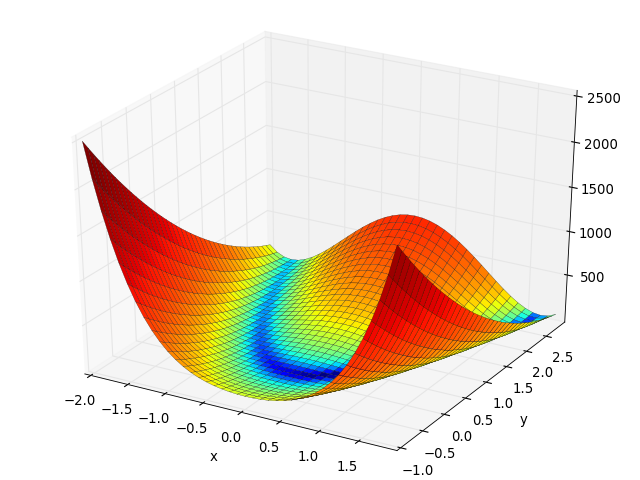
\includegraphics[height=7cm]{../figures/rosenbrock.png}
    \end{center}

\end{frame}

\begin{frame}[allowframebreaks]
    \frametitle{Results: ackley function}

    Average solution
    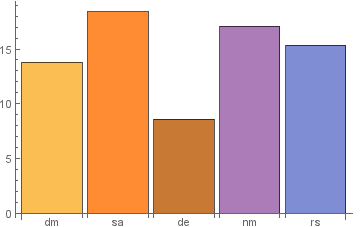
\includegraphics[width=5cm]{../figures/average-fun-ackley.png}

    Median solution
    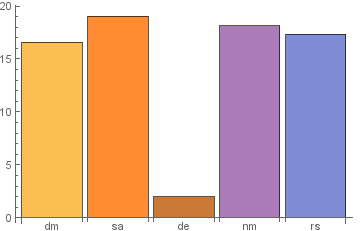
\includegraphics[width=5cm]{../figures/median-fun-ackley.png}

    Minimum solution
    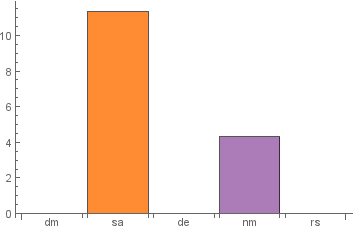
\includegraphics[width=5cm]{../figures/minimum-fun-ackley.png}
\end{frame}

\begin{frame}[allowframebreaks]
    \frametitle{Results: griewank function}

    Average solution
    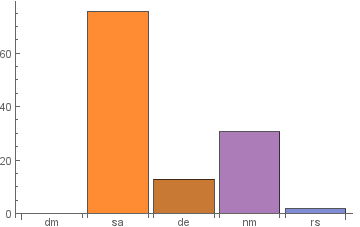
\includegraphics[width=5cm]{../figures/average-fun-griewank.png}

    Median solution
    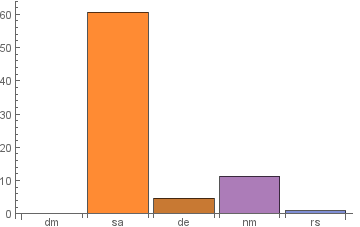
\includegraphics[width=5cm]{../figures/median-fun-griewank.png}

    Minimum solution
    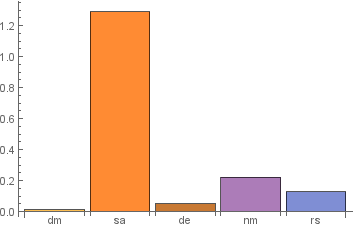
\includegraphics[width=5cm]{../figures/minimum-fun-griewank.png}
\end{frame}

\begin{frame}[allowframebreaks]
    \frametitle{Results: schaffer function}

    Average solution
    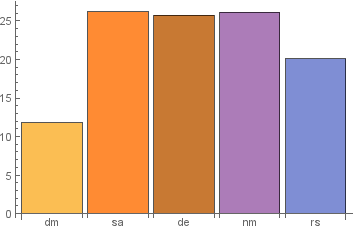
\includegraphics[width=5cm]{../figures/average-fun-schaffer.png}

    Median solution
    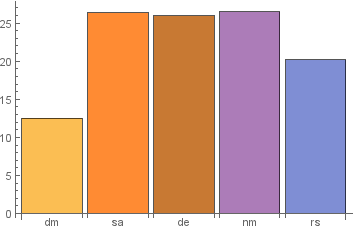
\includegraphics[width=5cm]{../figures/median-fun-schaffer.png}

    Minimum solution
    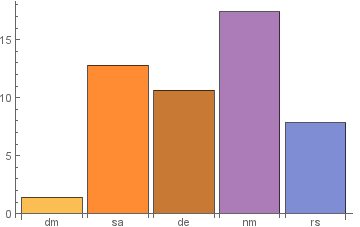
\includegraphics[width=5cm]{../figures/minimum-fun-schaffer.png}
\end{frame}

\begin{frame}[allowframebreaks]
    \frametitle{Results: rosenbrock function}

    Average solution
    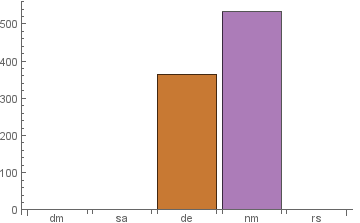
\includegraphics[width=5cm]{../figures/average-fun-rosenbrock.png}

    Median solution
    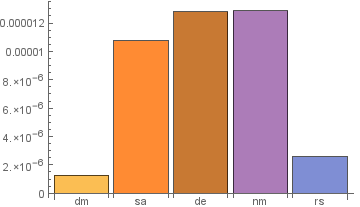
\includegraphics[width=5cm]{../figures/median-fun-rosenbrock.png}

    Minimum solution
    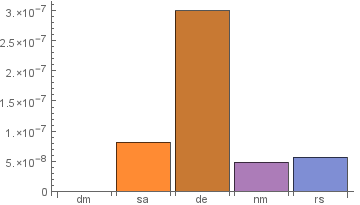
\includegraphics[width=5cm]{../figures/minimum-fun-rosenbrock.png}
\end{frame}

\end{document}
